
\documentclass[11pt]{article}
\usepackage[utf8]{inputenc}	% Para caracteres en español
\usepackage{amsmath,amsthm,amsfonts,amssymb,amscd}
\usepackage{multirow,booktabs}
\usepackage[table]{xcolor}
\usepackage{fullpage}
\usepackage{lastpage}
\usepackage{enumitem}
\usepackage{fancyhdr}
\usepackage{mathrsfs}
\usepackage{wrapfig}
\usepackage{setspace}
\usepackage{calc}
\usepackage{multicol}
\usepackage{cancel}
\usepackage[retainorgcmds]{IEEEtrantools}
\usepackage[margin=3cm]{geometry}
\usepackage{amsmath}
\newlength{\tabcont}
\setlength{\parindent}{0.0in}
\setlength{\parskip}{0.05in}
\usepackage{empheq}
\usepackage{framed}
\usepackage[most]{tcolorbox}
\usepackage{xcolor}
\colorlet{shadecolor}{orange!15}
\parindent 0in
\parskip 12pt
\geometry{margin=1in, headsep=0.25in}
\theoremstyle{definition}
\newtheorem{defn}{Definition}
\newtheorem{reg}{Rule}
\newtheorem{exer}{Exercise}
\newtheorem{sln}{Solution}
\newtheorem{note}{Note}
\begin{document}
\setcounter{section}{0}
\title{Lectuers 3,4,5 Important notes}

\thispagestyle{empty}
\begin{center}
\textsc{\LARGE German University in Cairo}\\[1.0cm]
{\LARGE \bf Lectures 18}\\ [0.5cm]
{\large \bf Math301}\\ [0.5cm]
Fall 2020
\end{center}
\tableofcontents
\section{Lecture 3}
\begin{reg}
Clairaut's Thm.
\end{reg}
\textbf{if the functions $Fxy$ and $Fyx$ are countinous on an open Disk D}
\begin{equation}
	F_{xy}=F_{yx}
\end{equation}
\begin{note}
	Please note that clairaut's thm. hold for any number of variables, that is $f_{zh} = f_{hz}$. So it's true for any two vars. (2nd partial derivative)
\end{note}
\begin{reg}
Direction vector from a slope
\end{reg}
Recall that if m = slope of the tangent line, then:
\begin{equation}
	v = (1,m)
\end{equation}
\begin{reg}
Same goes with partial derivatives:
\end{reg}
\begin{align}
	V1 = (1,0,\frac{\partial f}{\partial x}) &&
V2= (0,1,\frac{\partial f}{\partial y})
\end{align}
\begin{note}
	the zero in the aforementioned vectors comes from defferentiating with respect to a constant :) as we all know that in order to partial defferentiate you fix one variable and diff wrt to the other.

\end{note}
\begin{reg}
Find the partial derivatives:
\end{reg}
in these questions we find $f_x, f_y, f_z$ and so on.
\begin{reg}
Find the mixed partial derivatives:
\end{reg}
now we find $f_{xx}, f_{yy}, f_{xy}, f_{yx}$
\begin{reg}
	The meaning/interpretation of $\frac{\partial f}{\partial w}$, where w is any varibale{$x,y,z$}.
\end{reg}
The instantaous change of $f$ with respect to $w$ while holding all the other variables fixed.
\begin{reg}
Find a tangent plane to a surface:
\end{reg}
We know that a two varibale function's graph is a surface or a shape in space. We also knew how to get two tangent lines/vectors to surface at any point.\\
So Assuming that the surface is \textbf{Smooth} and has no peakes: a normal to the surface at that same point can be optained:
\begin{equation}
	n = V1 \times V2 = \begin{vmatrix}
		i & j & k \\
		1 & 0 & \frac{\partial f}{\partial x}\\
		0 & 1 & \frac{\partial f}{\partial y}
	\end{vmatrix} = (-f_x, -f_y, 1)
\end{equation}
and now the equation of the plane is 
\begin{equation}
	PM . n = 0
\end{equation}
that makes sense because n is normal to any vector in the plane. M is any point that belongs to the plane so $M=(x,y,z)$\\
and finally the equation of the plane is:
\begin{equation}
	z = f(a,b) + f_x(a,b)*(x-a) + f_y(a,b)*(y-b)
\end{equation}
\begin{reg}
	find Linear Approximation of a two variable function:
\end{reg}
Tangent planes that we studied now provide a good approximation of the original function at that point, same as we did with linear approximation in one var functions; the tangent line assumes a near value to the function.\\
Hence, we use tangent planes to find Linear approxiamtions:
\begin{equation}
	L(a,b) = f(a,b) + f_x(a,b)*(x-a) + f_y(a,b)*(y-b)
\end{equation}
For (x,y) $\approx$ (a,b) (very close to)
\begin{reg}
Using differentials and linearzation
\end{reg}
we use them together in order to find the difference between two close values of the real function. smth like finding the error of calculating volume of box, The inputs (x,y,z) has two valuse x1,x2 y1,y2 z1,z2 .\\
However, using \textbf{$L(a,b,c) = f(a,b,c) + f_x(a,b,c)*(x-a) + f_y(a,b,c)*(y-b) + f_z(x,y,z)*(z-c)$ together with $\Delta f = f(x,y,z) - f(a,b,c)$ 
and $f(x,y,z) \approx L(x,y,z)$\\}
We find that;
\begin{equation}
	\Delta f \approx df = f_x(x-1) + f_y(y-b) + f_z(z-c)
\end{equation}
it's the same as L but without the function at that point $f(a,b,c)$
\section{Lecture 4}
\begin{reg}
Solving problems including chain rule is just drawing a tree diagram:
\end{reg}
\begin{center}
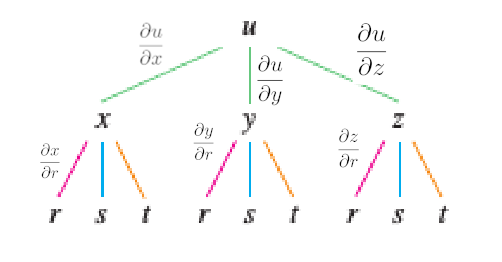
\includegraphics[scale=0.5]{images/tree.png}
\end{center}
after drawing the dependecy tree as show, solve! \\
for example: 
\begin{exer}
	Find $\frac{\partial u}{\partial r}$
\end{exer}
\begin{sln}
\begin{equation}
	\frac{\partial u}{\partial r} = \frac{\partial u}{\partial x} * \frac{\partial x}{\partial r} + \frac{\partial u}{\partial y} * \frac{\partial y}{\partial r}+ \frac{\partial u}{\partial z}* \frac{\partial z}{\partial r} 
\end{equation}
\end{sln}
\begin{note}
please note that 
\begin{equation}
	\frac{\partial^2 f}{\partial x \partial y } = \frac{\partial }{\partial x} [ \frac{\partial f}{\partial y }] = f_{yx}
\end{equation}
The notation is just inverted 
\end{note}
\begin{reg}
Directional Derivatives ?
\end{reg}
When we get $ \frac{\partial f}{\partial x} $ we try to find the derivative of $f$ with respect to $x$ or in the $x$ direction. 
\\ but what if we want to get the Directional derivative in any other direction $u=(u_1, u_2)$ or wrt to any other variable ? Note that that variable is a combination of the original variables. \\ 
However:
\begin{equation}
	D_u(f(a,b)) = \frac{d}{ds} |_{s=0} f(a+su_1, b+su_2)
\end{equation}
this rule is a bit amibgious so lets look at the easy form of it
\begin{equation}
	D_u(P_0)=\bf  \nabla f . u 
\end{equation}
\begin{reg}
Gradient Vectors
\end{reg}
\begin{equation}
	\nabla f = ( \frac{\partial f}{\partial x}, \frac{\partial f}{\partial y} ) = \frac{\partial f}{\partial x} i + \frac{\partial f}{\partial y} j
\end{equation}
and for the 3d case it's the same but we add another variable, hence another term in the vector in k direction \\

So the directional derivative is simply a\textbf{ dot product} of the gradient vector and a unit vector in the direction we need.\\
\begin{reg}
The magnitude of change and its significance 
\end{reg}
\begin{equation}
	|D_u| = |\nabla f| * |u| * cos(\theta)
\end{equation}
\begin{enumerate}

\item At any point $P_0$ the function f increases most rapidly in the direction where $\theta = 0$ or equally in the direction of the gradient vector.
\\ this also means that $u // \nabla f$ and $|D_u=|\nabla f |$
\item Simialrly, $f$ decreases most rapidly in the direction where $\theta = \pi$ so that $|D_u| = -|\nabla f|$
\item lastly f faces no change when $\theta = \frac{\pi}{2}$ so that $|D_u| = 0$ and $\nabla f$ is prepinduclar to $u$
\end{enumerate}
\begin{reg}
	How to find the normal to any given vector ?
\end{reg}
\begin{equation}
	\text{let }   v.u =0
\end{equation}
and solve it algebriaclly then you find v
\begin{reg}
\textbf{Gradient Vectors} are normal to \textbf{Level Curves}
\end{reg}
The proof is simple; we know that level curves are obtained when $f=k$ so when $f$ is constant. Constant means there is no change an hence from the above rule and third point in the list, We conclude that the grad. vector is prep. to the curve which is a level curve.\\
So \textbf{Gradient Vectors} are also prep. to \textbf{Level Surfaces} in case of a three variable function.
\begin{note}
A function of one variable can be thought of as a level curve to another function of two variables. HOW? \\
\begin{align}
	y = x^2 \text{  This is a normal function of one var} \\
	f= y-x^2 = 0 \text{  This is a level curve of another function f=k where k =0 }
\end{align}
Same goes with a function of two variables can be thought of as a level surface of another function.
\begin{align}
z^2 = x^2 + y^2 \\
f = x^2 + y^2 - z^2=0
\end{align}
why we did that ? 
in order to find a unit normal to the graph of z we can get it using $n=u_1 \times u_2$ and find $u_1, u_2$ using the rule no. 7 \\
or simply we can make it a level surface and then finding $\nabla f$ is just that easy.
\end{note}
\begin{reg}
unit vectors to level surfaces point downward or upward?
\end{reg}
you know that by looking at the components of the gradient vector or simply draw that gradient/unit normal in a 3d plane and look at it
\section{Lecture 5}
\begin{reg}
	Function optimization (finding local and absolute extrema points)
\end{reg}
To find the extrema points we have two methods
\begin{enumerate}

\item First derivative test
\item Lagrange Multiplier

\end{enumerate}
\begin{reg}
First Derivative Test 
\end{reg}
you find solutions of the following equations :
\begin{equation}
	\nabla f= 0 
\end{equation}
Which is equally
\begin{align}
	f_x=0\\f_y=0\\f_z=0
\end{align}	
The solution of those equations gives us \textbf{Critical} points
\begin{reg}
Checking if critical points are local max/min using Second deriv. Test
\end{reg}
\begin{equation}
	D(a,b) = f_{xx}(a,b) *f_{yy} (a,b) - [f_{xy}](a,b) ^2
\end{equation}
\begin{enumerate}

\item if $D>0$
	\begin{enumerate}
	
		\item if $f_{xx}<0$ f has a local maximum point at (a,b)
		\item  if $f_{xx}>0$ f has a local minimum extrema at (a,b) 
	
	\end{enumerate}
\item $D<0$ Then the point is a saddle point (not local max nor min)
\item $D=0$ Then the test fails

\end{enumerate}
\begin{reg}
	What is $D$ ? it's called the \textbf{Hessian} or the \textbf{Discriminant} of the function f
\end{reg}
\begin{equation}
	D = \begin{vmatrix}
		f_{xx} & f_{yy} \\
		f_{yx} & f{yy}
	\end{vmatrix}
\end{equation}
\begin{note}
	This first derivative test is used to find critical points which are inside the domain of f, not on the boundary of that domain. At the boundary you either use another method or find it by substitution and some math \textbf{please look at the following example}
\end{note}
	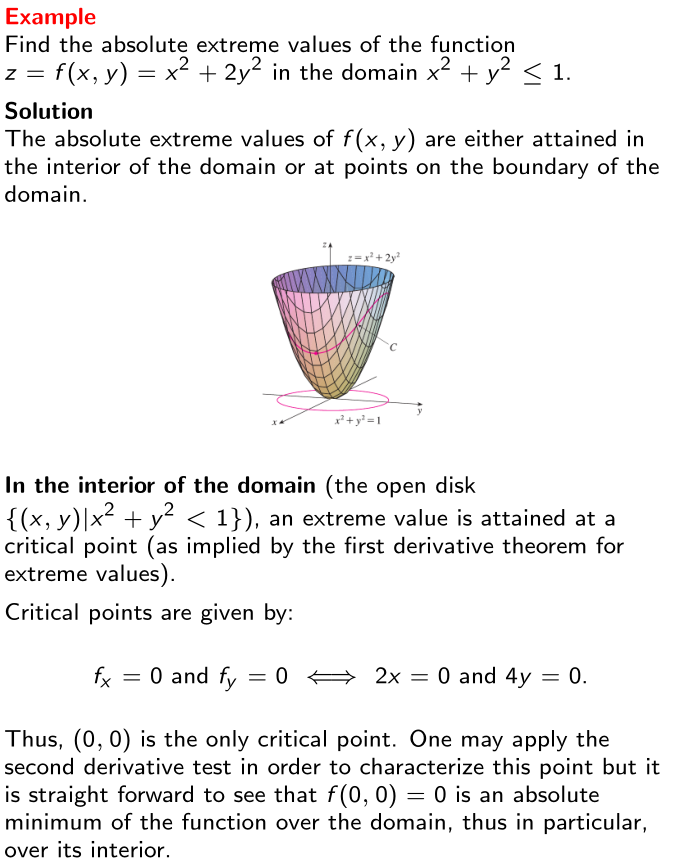
\includegraphics[scale=0.4]{images/q1.png} 
	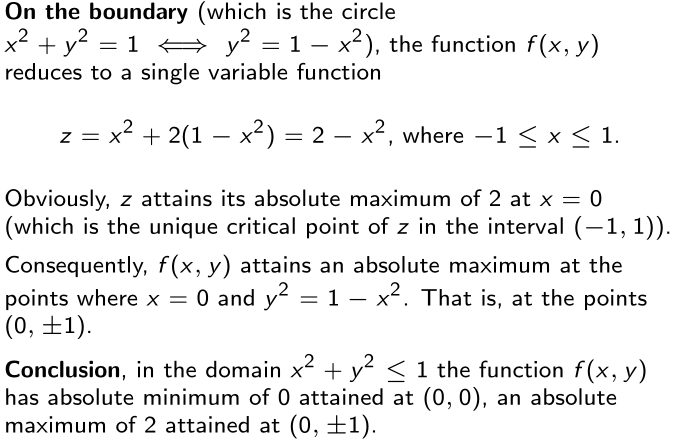
\includegraphics[scale=0.4]{images/q1-1.png}
\begin{reg}
Method of lagrange multipliers
\end{reg}
This method is used when you have a constraint (like the previous boundary problem)
\begin{align}
	\nabla f(x,y) = \lambda \nabla g(x,y) \\
	g(x,y) = k
\end{align}
Solving the two equations together and finding $\lambda$ will yield solutions for the critical points \\
your goal is to find all the values of $x,y,\lambda$ that satisfies the equations and then substitue with those points
\begin{enumerate}

\item the point that yields the largest value of f is a maximum value
\item same with the smallest is the minimum value 

\end{enumerate}

\end{document}
